\newpage
\section{Analisi dei rischi}

Al fine di ridurre al minimo i possibili ritardi sulla pianificazione e migliorare la qualità del progetto, vengono di seguito analizzati i rischi che potrebbero insorgere nel corso dello sviluppo.\\
Per ogni rischio è associata un'analisi dettagliata, così suddivisa:

\begin{itemize}
	\item \textbf{Identificazione:} viene individuata la natura del rischio e ne viene data una sintetica descrizione.
	\item \textbf{Analisi:} si fornisce la probabilità stimata di insorgenza ed il livello di gravità ad essa associata.
	\item \textbf{Pianificazione:} viene definito un piano d'azione in modo da rendere minima la probabilità di insorgenza del rischio. 
	\item \textbf{Contenimento:} nel caso in cui il rischio, nonostante le misure adottate, dovesse comunque insorgere, viene già deciso come agire per contenerlo.
\end{itemize}

È possibile prendere visione dei rischi che si sono effettivamente riscontrati durante le varie fasi di sviluppo nell'\hyperref[RiscontroRischi]{Appendice A}\\
Di seguito la tabella con i rischi individuati, divisi a seconda del livello di appartenenza:\\

\begin{center}
	\centerline{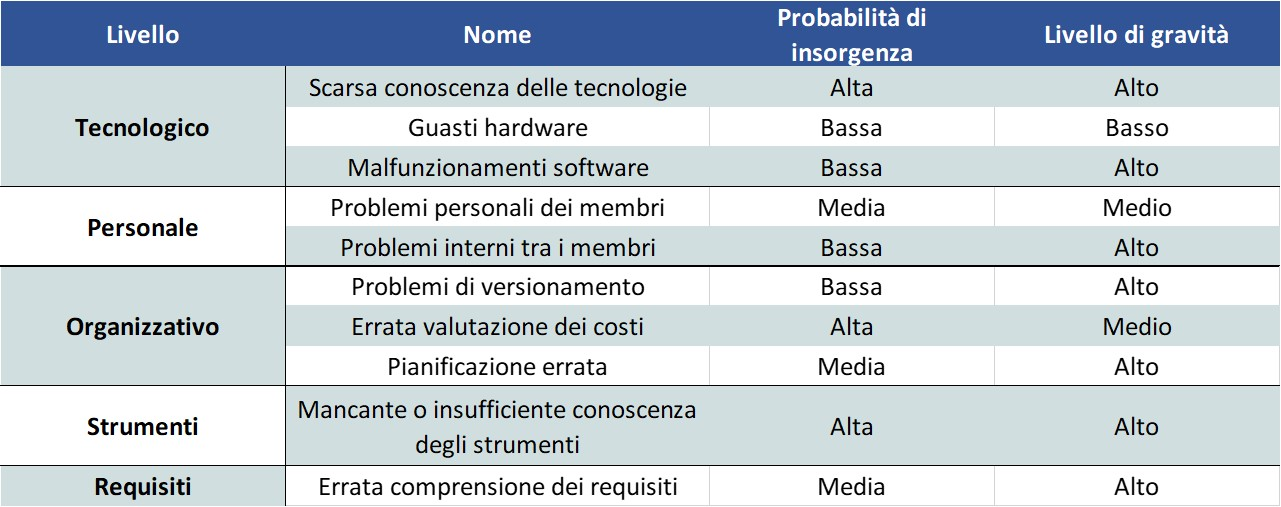
\includegraphics[scale=0.50]{img/TabellaRischi.jpg}}
\end{center}

\subsection{Livello tecnologico}
\subsubsection{Scarsa conoscenza delle tecnologie}

\paragraph {Identificazione}
Alcune delle tecnologie utilizzate sono sconosciute a uno o più membri del gruppo, mentre altre sono state viste solo in ambito teorico. In generale, esistono tecnologie con cui il gruppo non ha il grado di dimestichezza richiesto.

\paragraph {Analisi}
\begin{itemize}
	\item \textbf{Probabilità di insorgenza:} Alta.
	\item \textbf{Livello di rischio:} Alto.
	\item \textbf{Possibili conseguenze:} ritardi nei tempi prestabiliti, un maggiore numero di errori.
\end{itemize}

\paragraph {Pianificazione}
I membri del gruppo si impegnano a documentarsi in modo autonomo e responsabile. Saranno seguiti dagli Amministratori, che forniranno le documentazioni necessarie e si cercherà di condividere il più possibile le conoscenze di ognuno dei membri del gruppo.

\paragraph {Contenimento} Nel caso in cui dovessero comunque presentarsi problemi, il Responsabile di Progetto provvederà a sollevare momentaneamente il membro carente dal proprio incarico per permettergli di aggiornarsi nel minor tempo possibile. 

\subsubsection{Guasti hardware}
\paragraph {Identificazione}
Viene tenuto conto di possibili guasti dei dispositivi utilizzati per lavorare dei membri del gruppo. Si includono possibili malfunzionamenti di PC e problemi alla linea internet.

\paragraph {Analisi}
\begin{itemize}
	\item \textbf{Probabilità di insorgenza:} Bassa.
	\item \textbf{Livello di rischio:} Basso.
	\item \textbf{Possibili conseguenze:} ritardi nei tempi prestabiliti, possibile perdita del lavoro temporaneo svolto.
\end{itemize}

\paragraph {Pianificazione}
Per evitare perdita di dati significativi, i membri del gruppo eseguiranno backup regolari su repository. In caso di guasti i componenti del gruppo si impegnano a proseguire il proprio lavoro tramite un altro dispositivo personale o uno presente nelle aule informatiche dell'università.

\paragraph {Contenimento}
Se dovessero insorgere dei problemi si provvederà a recuperare la versione aggiornata del materiale da repository.	Il membro interessato potrà utilizzare gli altri dispositivi sopracitati nel tempo necessario alla riparazione/sostituzione.

\subsubsection{Malfunzionamenti software}
\paragraph {Identificazione}
È possibile che, nel corso del progetto, i software utilizzati incorrano in dei malfunzionamenti che potrebbero causare perdita di dati o incompatibilità tra versioni in possesso di membri diversi.

\paragraph {Analisi}
\begin{itemize}
	\item \textbf{Probabilità di insorgenza:} Bassa.
	\item \textbf{Livello di rischio:} Alto.
	\item \textbf{Possibili conseguenze:} ritardi nei tempi prestabiliti, impossibilità o ritardi per un membro di completare il proprio compito, possibile perdita di dati significativi.
\end{itemize}

\paragraph {Pianificazione}
Oltre alle strategie di backup già illustrate precedentemente, gli Amministratori si impegnano a garantire che tutti i membri del gruppo dispongano della stessa versione del software.

\paragraph {Contenimento}
Qualora un membro dovesse rilevare problemi software provvederà a comunicarlo tempestivamente agli Amministratori; qualora il problema riguardasse invece l'intero gruppo, spetterà al Responsabile decidere se cambiare software o utilizzarne un'altra versione, previo consulto con gli Amministratori.

\subsection{Livello personale}
\subsubsection{Problemi personali dei membri}
\paragraph {Identificazione}
Vengono presi in considerazione gli eventi imprevisti che potrebbero influire sulla disponibilità dei membri del gruppo, come per esempio periodi di malattia o complicazioni famigliari.

\paragraph {Analisi}
\begin{itemize}
	\item \textbf{Probabilità di insorgenza:} Media.
	\item \textbf{Livello di rischio:} Medio.
	\item \textbf{Possibili conseguenze:} ritardi nei tempi prestabiliti.
\end{itemize}

\paragraph {Pianificazione}
I membri del gruppo, sfruttando i canali di comunicazioni predisposti, provvederanno ad informare tempestivamente i propri colleghi. Nel caso in cui l'indisponibilità del componente si prolungasse, il Responsabile provvederà a ridurre il carico lavorativo e a modificare la pianificazione. Per arginare questo rischio sono stati previsti, ove possibile, dei periodi di slack.

\paragraph {Contenimento}
Qualora dovessero insorgere problemi, il Responsabile di Progetto ripartirà il lavoro, andando a sfruttare, se necessario, i periodi di slack prestabiliti. 

\subsubsection{Problemi interni tra i membri}
\paragraph {Identificazione}
Per ogni componente del gruppo è la prima esperienza di lavoro in un gruppo di grandi dimensioni. Tale fattore potrebbe causare problemi di collaborazione causando squilibri interni, provocando così dei ritardi nei lavori ed un clima non proficuo.

\paragraph {Analisi}
\begin{itemize}
	\item \textbf{Probabilità di insorgenza:} Bassa.
	\item \textbf{Livello di rischio:} Alto.
	\item \textbf{Possibili conseguenze:} ritardi nei tempi prestabiliti, blocco delle attività, peggioramento dell'ambiente lavorativo.
\end{itemize}

\paragraph {Pianificazione}
I membri del gruppo si impegnano a tenere un atteggiamento responsabile e maturo, andando subito a esternare eventuali dissapori tra loro e conferendo con il Responsabile di Progetto quando non riescano a gestire le loro incompatibilità.

\paragraph {Contenimento}
Se dovessero sorgere problemi per cui sia necessario l'intervento del Responsabile di Progetto, questi cercherà di appianare le divergenze e, se necessario, provvederà a riorganizzare il lavoro, separando i membri coinvolti.

\subsection{Livello organizzativo}
\subsubsection{Problemi di versionamento}
\paragraph {Identificazione}
Poiché i membri del gruppo non hanno mai lavorato prima a progetti così complessi e che richiedessero coordinazione tra tante persone, esiste la possibilità che si creino problemi di versionamento quando più persone sono incaricate di redigere o verificare lo stesso documento o la stessa parte di codice.

\paragraph {Analisi}
\begin{itemize}
	\item \textbf{Probabilità di insorgenza:} Bassa.
	\item \textbf{Livello di rischio:} Alto.
	\item \textbf{Possibili conseguenze:} ritardi nei tempi prestabiliti, confusione ed errori.
\end{itemize}

\paragraph {Pianificazione}
È stato predisposto un tracker in modo che ogni cambiamento sia sempre notificato e controllato. Il Responsabile di Progetto fornisce una divisione di ruoli che i membri si impegnano a seguire senza accavallarsi.

\paragraph {Contenimento}
In caso di problemi si provvederà e recuperare l'ultima versione corretta da repository.

\subsubsection{Errata valutazione dei costi}
\paragraph {Identificazione}
Poiché i membri del gruppo non hanno esperienze precedenti, è possibile che, nella fase di pianificazione, vengano sottostimati i costi, non solo economici, ma anche in termini di tempo.

\paragraph {Analisi}
\begin{itemize}
	\item \textbf{Probabilità di insorgenza:} Alta.
	\item \textbf{Livello di rischio:} Medio.
	\item \textbf{Possibili conseguenze:} ritardi nei tempi prestabiliti.
\end{itemize}

\paragraph {Pianificazione}
Il Responsabile di Progetto terrà sempre sotto controllo lo stato di avanzamento delle varie fasi rispetto alla pianificazione iniziale. Dove possibile andrà a sfruttare i periodi di slack predisposti, eventualmente ripianificando il lavoro del gruppo.

\paragraph {Contenimento}
In caso di ritardi il lavoro verrà ripianificato, cercando di rientrare nei tempi stabiliti.

\subsubsection{Pianificazione errata}
\paragraph {Identificazione}
Durante la pianificazione è possibile che i tempi per l'esecuzione di alcune attività vengano calcolati in modo errato.

\paragraph {Analisi}
\begin{itemize}
	\item \textbf{Probabilità di insorgenza:} Media.
	\item \textbf{Livello di rischio:} Alto.
	\item \textbf{Possibili conseguenze:} ritardi nei tempi prestabiliti.
\end{itemize}

\paragraph {Pianificazione}
La caratteristica dinamica del rischio impone che si debba controllare lo stato delle attività periodicamente, in modo da accertarsi dell'avanzamento previsto nello svolgimento dei vari task e verificare eventuali ritardi nello sviluppo di questi.

\paragraph {Contenimento}
Per ogni attività, il Responsabile di Progetto, prevederà un periodo maggiore di quanto normalmente richiesto, in modo tale che un eventuale ritardo non influenzi la durata totale del progetto.

\subsection{Strumenti}
\subsubsection{Mancante o insufficiente conoscenza degli strumenti}
\paragraph {Identificazione}
Lo sviluppo del progetto richiede l'utilizzo di vari strumenti mai utilizzati prima dal gruppo o il cui uso non è stato esaustivo.

\paragraph{Analisi}
\begin{itemize}
	\item \textbf{Probabilità di insorgenza:} Alta.
	\item \textbf{Livello di rischio:} Alto.
	\item \textbf{Possibili conseguenze:} ritardi nei tempi prestabiliti, rallentamenti nelle varie attività.
\end{itemize}

\paragraph {Pianificazione}

Ogni volta che sarà ritenuto necessario, dal Responsabile di progetto e dagli Amministratori, utilizzare un nuovo strumento, tutti i membri del gruppo verranno subito avvertiti. L'introduzione di nuovi strumenti sarà sempre una scelta pesata e responsabile, consapevole degli alti livelli di rischio che può comportare. \\
Una volta introdotto tale strumento, il gruppo si dovrà documentare su come impiegarlo al meglio seguendo le indicazioni fornite dall’Amministratore.

\paragraph {Contenimento}
Se tutti i membri del gruppo dovessero riscontrare gravi difficoltà nell'apprendimento di uno strumento, o se il Responsabile riterrà i tempi di apprendimento troppo lunghi, si opterà per la selezione di un altro strumento più adatto.

\subsection{Requisiti}
\subsubsection{Errata comprensione dei requisiti}
\paragraph{Identificazione}
Si preventiva una mancata comprensione tra il gruppo e il proponente, che può portare a inesattezze nei requisiti e nella comprensione del prodotto che il proponente e il committente si aspettano.

\paragraph{Analisi}
\begin{itemize}
	\item \textbf{Probabilità di insorgenza:} Media.
	\item \textbf{Livello di rischio:} Alto.
	\item \textbf{Possibili conseguenze:} ritardi nei tempi prestabiliti, rallentamenti nelle varie fasi, possibilità di dover tornare sui propri passi.
\end{itemize}

\paragraph {Pianificazione}
Si è cercato di ridurre al minimo la possibilità di insorgenza di questo rischio confrontandosi col proponente e col committente. Soprattutto nella fase di Analisi dei Requisiti, si vuole rendere il proponente partecipe, chiedendo spesso il suo parere ed il suo feedback.

\paragraph {Contenimento}
Per ogni dubbio, sarà necessario un confronto con il proponente in modo da poter definire con chiarezza ogni requisito necessario al corretto sviluppo del progetto. Sarà inoltre indispensabile correggere eventuali errori o imprecisioni indicati dal committente all’esito di ogni revisione.